% !TEX root =../thesis-letomes.tex

\chapter{Discussion}

\section{Stability of Trajectories: Lyapunov Exponent}
argue for correctness of method and trustworthiness of trajectories by quantifying the inherent chaos: Basically, we are addressing the fact that this is a numerical simulation, and therefore a compressed view of the real thing. It is important to argue that that compression is not too much.

\subsection{Sensitivity analysis}

In our experiments, we found that our paths were diverging pretty heavily given relatively small changes to initial conditions. This was a concern in the original project as well, but was not fully explored then. It is important to quantify the chaotic nature of a system like this, since we are dealing with numerical simulation, which will always have some error associated with it. One takes steps to minimize such errors, often sacrificing computing performance to do so. However, if a system has an error of magnitude say \(\num{1e-8}\), and the system is so chaotic that errors of or \(\num{1e-9}\) at one point early in the trajectory effect meaningful changes further down the line, then the path is near invalid! Therefore, it is important to try to quantify the chaos of a system (in this case our simulator), to provide assurances that the resulting paths have any meaningful truth to them. We have done this by calculating Lyapunov exponents for the system, explained below.

\subsection{Lyapunov Exponent}

The Lyapunov exponent describes the rate of change as time goes on between time series with infinitesimally different starting conditions, as they progress. The method is to compute a set of trajectories, and take the difference between them at set points in time (euclidean distance when dealing with higher dimensions). In a chaotic system, these two trajectories should diverge from each other at some exponential rate, and the Lyapunov exponent is that rate. If we want to trust our results, we want that number to be as low as possible. 

\subsection{Implementation}

We ran several simulations of known good trajectories, with their starting conditions very slightly perturbed, in such a way that the trajectories initially diverged from each other by a value less that 1e-8, chosen as the square root of the precision of the 64-bit floating point numbers that describe the coordinates. The trajectories were then discretized to synchronize the variable length of the time steps, and then compared in pairs, tick by tick, yielding a list of euclidean distances at each step. We then took the natural logarithm of these lists, giving us the plots pictured in figure \ref{fig:long_leto_slope} and \ref{fig:hohmann_slope}. The graph varied heavily depending on the gist of the trajectory in question, with trajectories that made multiple passes near earth giving the tooth-like distance graphs pictured in fig. \ref{fig:long_leto_slope}. Trajectories that did not visit earth more than once gave much more `normal' results, given what we see in the literature pertaining to Lyapunov exponent analysis. Clearly, passing into the LEO domain has a powerful stabilizing effect on the the chaotic system, acting like a focal lens for the trajectories passing through. It's not completely trivial to give a Lyapunov exponent from this, but since the individual tooth-segments have a more or less equivalent slope, we simply took the average slope of all the teeth. A deeper look into this cyclical chaos would be interesting, but we will not delve deeper than this.

A good heuristic for whether or not our paths are precise enough would be a measure that would give some confidence interval for final position, given the gist of a trajectory, and the duration of flight along it. We have calculated such measures, presented in fig. \todoref{reflyapunov heuristic}.

\begin{figure}
    \centering
    \subfloat[a straight-forward Hohmann transfer]{
        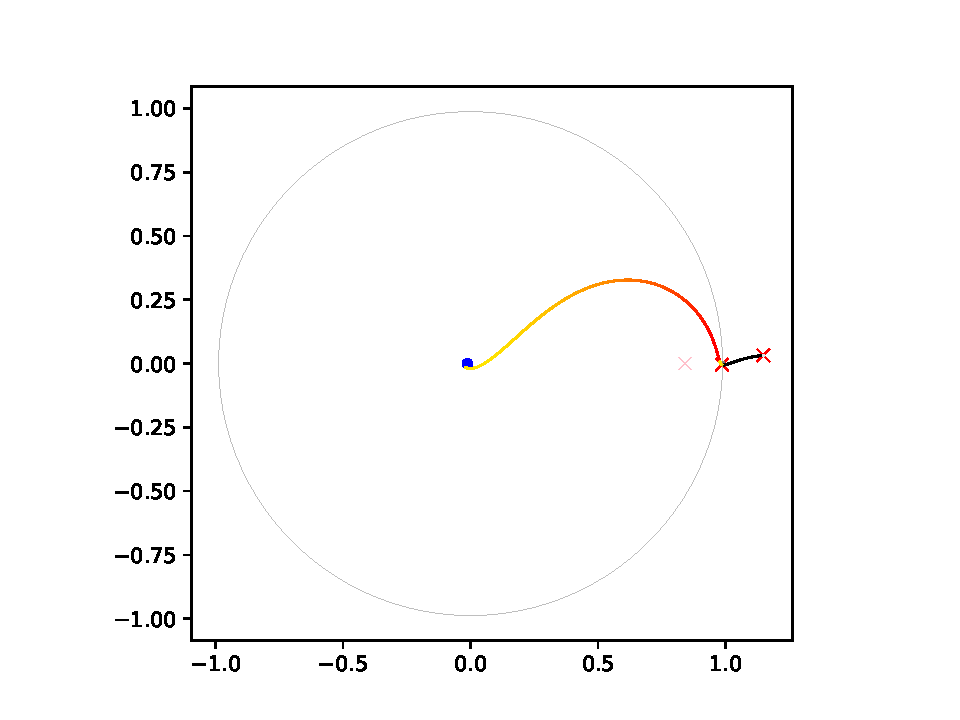
\includegraphics[width=0.46\linewidth]{fig/path_hohmann_nonin_multi_0_and_3}
        \label{fig:path_hohmann_non-inertial_multi}
    }
    \hfill
    \subfloat[the rate of separation between infinitesimally perturbed versions of the Hohmann transfer]{
        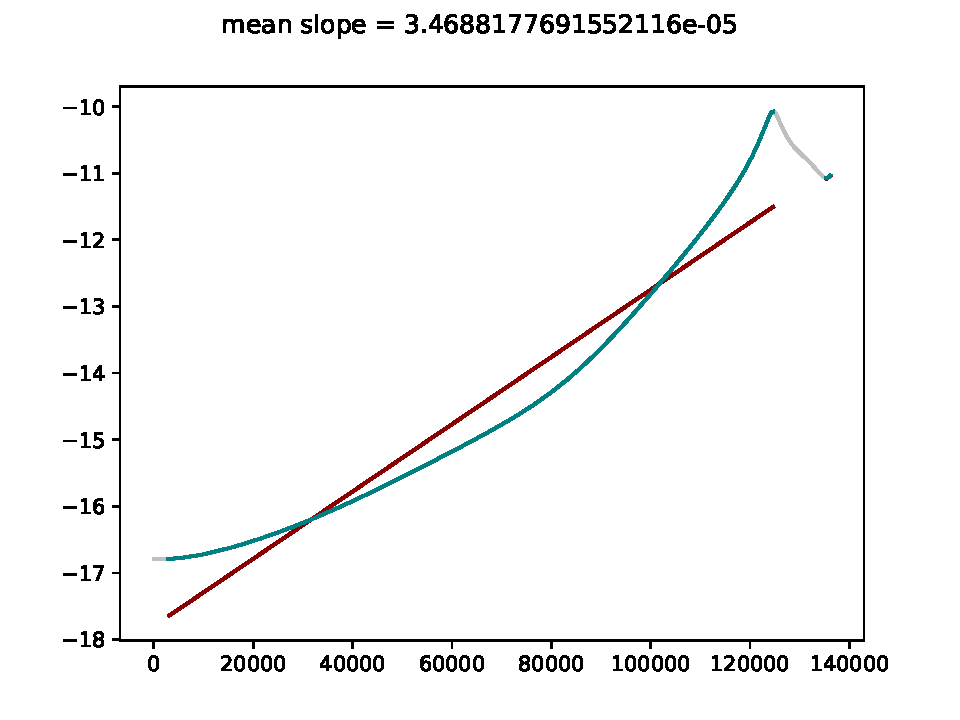
\includegraphics[width=0.46\linewidth]{fig/hohmann_slope_0_and_3}
        \label{fig:hohmann_slope}
    }
    \\
    \subfloat[a relatively long LETO path]{
        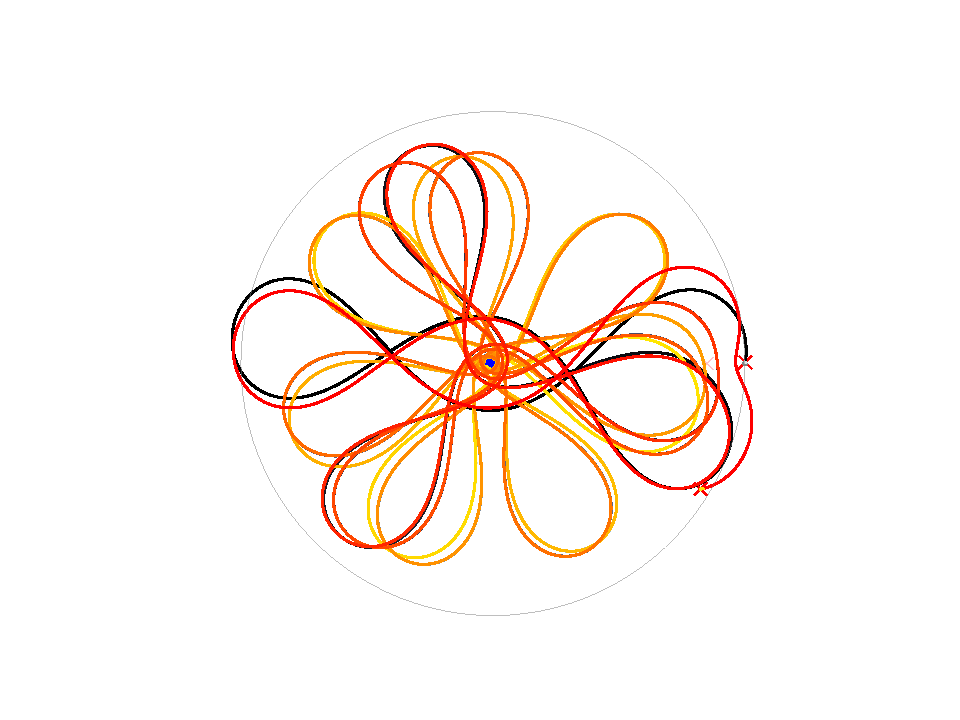
\includegraphics[width=0.46\linewidth]{fig/path_long_leto_nonin_multi_1_and_3}
        \label{fig:path_long_leto_non-inertial_multi}
    }
    \hfill
    \subfloat[the rate of separation of two infinitesimally perturbed versions of the long LETO]{
        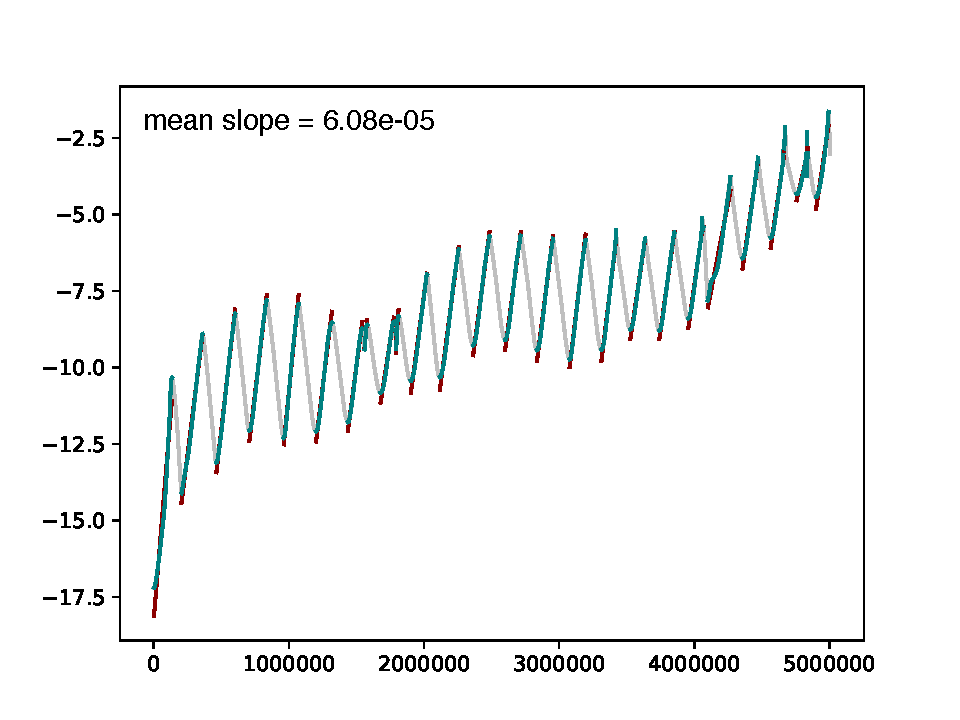
\includegraphics[width=0.46\linewidth]{fig/long_leto_slope_1_and_3}
        \label{fig:long_leto_slope}
    }
    \caption{Examples of some of the different types of transfers that are possible within the model. Each of these were taken as starting points, and simulated again with slightly perturbed starting conditions. The difference between these perturbations were then measured, and plotted in \textbf{b} and \textbf{d}, on a logarithmic scale. The slope of these plots is the lyapunov exponent. We can see that passing into a deep gravity well has a stabilizing effect on the chaos in the system.}
    \label{fig:lyapunov}
\end{figure} 

Our analysis shows that given an initial perturbation in the order of \num{1e-6}, after 200 days we have an uncertainty of 50.000 kilometers. This is a very liberal upper bound for both our error and our flight time. A definite confirmation that the system is significantly chaotic, but not enough to invalidate our results. 

A more reasonable initial perturbation on the order of \num{1e-8} (one order of magnitude greater than our error tolerance) gives us an uncertainty of less than \SI{2700}{km} after the same 200 days (before we pass the moon, which of course stops one path, and heavily diverges the other). This is very manageable for a spacecraft, since it can adjust for these imprecisions with its guidance thrusters early in the process.

The mean slope for our longer and shorter missions remain the same within a single order of magnitude, (\num{1e-5}-\num{1e-4}), which is encouraging. Our conclusion with regards to the chaos of the system is that it is significant, and will need to be corrected for dynamically in an actual mission, but that it does not invalidate any trajectories that we find, since the aforementioned dynamic corrections are completely covered by modern- (and to an extent, even vintage) spacecraft capabilities.


% \begin{figure}
%     \centering
%     \subfloat[test-a]{
%         
\includegraphics[width=0.46\linewidth]{temp/img1}
%         \label{img1}
%     }
%     \hfill
%     \subfloat[test-b]{
%         
\includegraphics[width=0.46\linewidth]{temp/img2}
%         \label{img2)}
%     }
%     \\
%     \subfloat[test-c]{
%         
\includegraphics[width=0.46\linewidth]{temp/img3}
%         \label{img3}
%     }
%     \hfill
%     \subfloat[test-d]{
%         
\includegraphics[width=0.46\linewidth]{temp/img4}
%         \label{img4)}
%     }
%     \caption{Overall caption}
%     \label{fig:somelabel}
% \end{figure} 

% \begin{figure}
%     \centering
%     \subfloat[Figure a) caption]{
%         
\includegraphics[width=0.46\linewidth]{temp/img1}
%         \label{fig:Image a) filename}
%     }
%     \hfill
%     \subfloat[Figure b) caption]{
%         
\includegraphics[width=0.46\linewidth]{temp/img2}
%         \label{Image b) filename)}
%     }
% \end{figure} 
%     \\
%     \centering
%     \subfloat[Figure c) caption]{
%         
\includegraphics[width=0.46\linewidth]{temp/img3}
%         \label{fig:Image c) filename}
%     }
%     \hfill
%     \subfloat[Figure d) caption]{
%         
\includegraphics[width=0.46\linewidth]{temp/img4}
%         \label{Image d) filename)}
%     }
%     \caption{field 1:default=Overall caption}
%     \label{fig:Overall figure label}
% \end{figure}


\section{Brute Force vs. ES}
In this section, we will examine the usefulness of using the ES algorithm over the brute force alternative. Do we get anything out of estimating a gradient? Do our results’ quality scale with a more complex model?

The ES method is in the general case a more intelligent of searching for these things. However, its not a magical panacea that just spits out fabulous results from a naive application. The brute force method took advantage of a lot of human intuition in terms of where to search. We gave it a limited fan of possibilities in a region that we knew to be reasonable. The ES algorithm definitely gave the best results when we imposed equivalent limitations on it.

\section{Delta-v Travel Time Trade-off}
Delta-v Travel Time Trade-off. Plot this, if we can get enough different successful trajectories. What does that plot look like?

\section{Performance Optimization}
Computing performance ended up representing a large portion of our efforts in this project, perhaps even more that we anticipated, and the tradeoff between code readability and performance was drawn in stark relief. We used several tools to make things easier: Initially, we wanted to get the parallelism 'for free' by using PaGMO to handle our multi-threading and use Numba to compile our python scripts. Seemed like a good idea; that's what the respective tools are made for. However, while Numba definitely gave fantastic performance increases over normal python, it was not enough. And while PaGMO worked fine (after some work getting it running at all), it only parallelized to CPUs, and had an absolutely hilarious startup overhead that made rapid prototyping (one of the main draws of python) tedious to say the least. 

In the end, we had to apply the adage of \textit{"if you want something done right, do it yourself"}, and implement these things by hand, with a C implementation of the integrator, and a CUDA interface for parallelization. This of course also meant redesigning the otherwise simple ES algorithm to fit the much less sophisticated data types that graphics cards work with. It was easily worth the effort. This new iteration of the program completes four orders of magnitude more fitness evaluations in roughly the same time, compared to its predecessor. It makes it reasonable to get results with \textit{some} confidence that the problem space is significantly explored. 

More performance would be nice, and definitely achievable, but we have hit a point of diminishing returns on further effort in this regard. The obvious possible improvements would be to reduce the number of variables that we save in the core integrator loop: We use 96 registers per parallel evaluation, which means that the card is memory capped at 25\% capacity. We could realistically expect a doubling in performance if we refactored the C integrator with this in mind. Again, we didn't bother with this, since the current speed is good \textit{enough}.

\section{Self-evaluation}
Was our time well spent? Did we gain anything from our "reinventing the wheel", re-implementing the lunar simulator? Should we have focused on running on the old code without delving into it?